\documentclass[12pt]{article}
\usepackage[width=16cm]{geometry}                % See geometry.pdf to learn the layout options. There are lots.
\geometry{letterpaper}                   % ... or a4paper or a5paper or ... 
%\geometry{landscape}                % Activate for for rotated page geometry
%\usepackage[parfill]{parskip}    % Activate to begin paragraphs with an empty line rather than an indent
\usepackage{graphicx}
\usepackage{amssymb}
\usepackage{amsmath}
\usepackage{aliases}
\usepackage{color}
\usepackage{url}

\usepackage{listings}
\usepackage{cancel}
\usepackage{textcomp}

\lstset{
   language=matlab,
   keywordstyle=\bfseries\ttfamily\color[rgb]{0,0,1},
   identifierstyle=\ttfamily,
   commentstyle=\color[rgb]{0.133,0.545,0.133},
   stringstyle=\ttfamily\color[rgb]{0.627,0.126,0.941},
   showstringspaces=false,
   basicstyle=\small,
   numberstyle=\footnotesize,
   numbers=none,
   stepnumber=1,
   numbersep=10pt,
   tabsize=2,
   breaklines=true,
   prebreak = \raisebox{0ex}[0ex][0ex]{\ensuremath{\hookleftarrow}},
   breakatwhitespace=false,
   aboveskip={0.1\baselineskip},
    columns=fixed,
    upquote=true,
    extendedchars=true,
% frame=single,
    backgroundcolor=\color[rgb]{0.9,0.9,0.9}
}

\title{Two dimensional heat equation}
\author{Praveen. C, Deep Ray, Jean-Pierre Raymond}
%\date{}                                           % Activate to display a given date or no date

\begin{document}



\maketitle
%\section{}
%\subsection{}


\section{The PDE model}
Let $z = z(x,y,t)$ denote the temperature. 
The shifted 2-D heat equation is given by
\[
z_t = \mu \Delta z + \alpha z, \quad (x,y) \in \Omega = (0,1) \times (0,1), \qquad t \in  [0,T]
\]
with boundary conditions
\[
z(x,0,t) = z(x,1,t) = 0, \quad z(1,y,t) = u(y,t), \qquad \df{z}{x}(0,y,t) = 0
\]
and initial condition
\[
z(x,y,0) = z_0(x,y)
\]
Here $\alpha \ge 0$ and $\mu > 0$. Let us denote the Dirichlet part of the boundary by $\Gamma_D$
\[
\Gamma_D = \{ y=0\} \cup \{ y=1\} \cup \{ x=1 \}
\]
the Neumann part as
\[
\Gamma_N = \{ x=0 \}
\]
and the part on which the control is applied as
\[
\Gamma_c = \{ x=1 \}
\]
\begin{figure}
\begin{center}
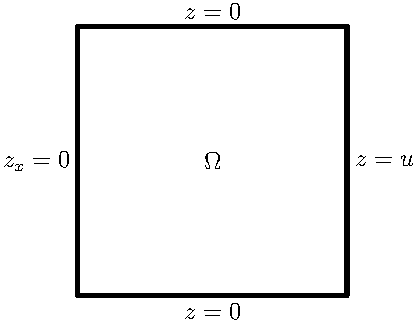
\includegraphics[width=0.5\textwidth]{heat2d_prob}
\caption{Problem definition}
\end{center}
\end{figure}
%------------------------------------------------------------------------------

\subsection{Observations}
We will measure an average value of the temperature on strips along the left vertical boundary
\[
I_i = [a_i, b_i]
\]
as shown in figure. Thus the observations are
\begin{equation}
y_i(t) = \frac{1}{b_i - a_i} \int_{a_i}^{b_i} z(0,y,t) \ud y
\end{equation}

\begin{figure}
\begin{center}
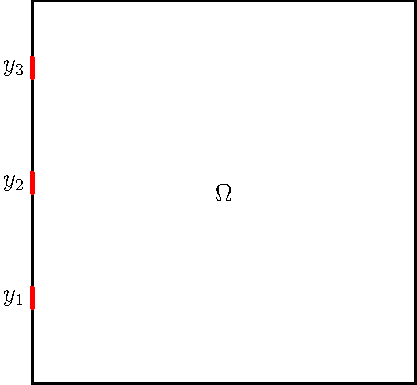
\includegraphics[width=0.5\textwidth]{heat2d_obs}
\caption{Observations}
\end{center}
\end{figure}
\noindent
{\bf Note}: Do not confuse the observation $y_i$ with the spatial coordinate $y$.
%------------------------------------------------------------------------------
\subsection{Weak formulation}
We assume $z_0 \in L^2(\Omega)$. We wish to find $z \in L^2(0,T;H^1(\Omega))$ such that
\[
 \dd{}{t}(z(t), \phi)_{L^2} = - \mu \int_\Omega \nabla z \cdot \nabla \phi \ud x +  \alpha \int_\Omega z \phi \ud x, \quad \forall \phi \in H^1_{\Gamma_D}(\Omega)
\]
\[
z(x,0,t) = z(x,1,t) = 0, \quad z(1,y,t) = u(y,t)
\]
\[
 (z(0),\phi)_{L^2} = (z_0 ,\phi)_{L^2}
\]
%------------------------------------------------------------------------------

\section{FEM approximation}
\begin{figure}
\begin{center}
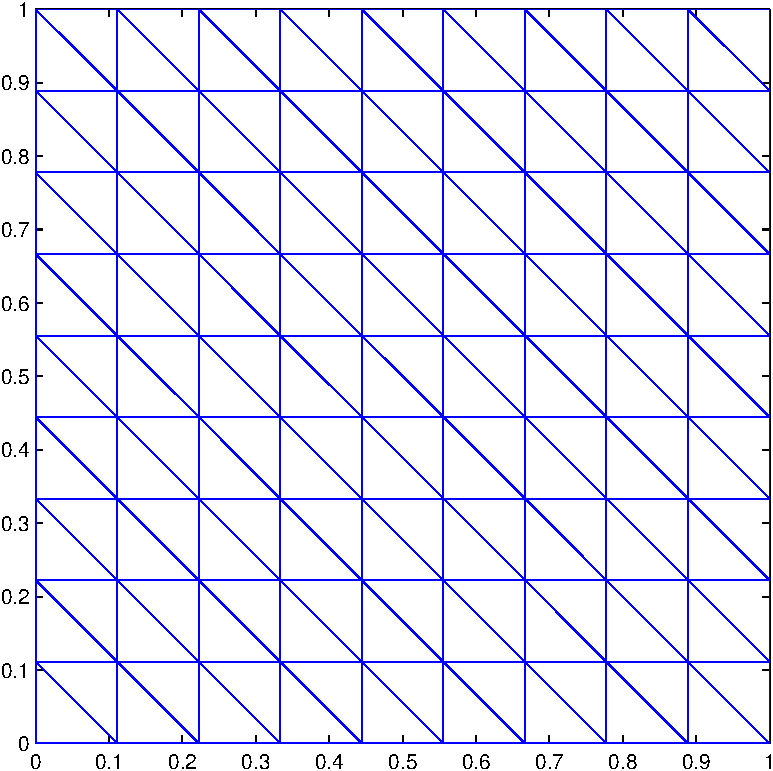
\includegraphics[width=0.5\textwidth]{heat2d_mesh}
\caption{Example of a finite element mesh}
\end{center}
\end{figure}
Consider a division of $\Omega$ into disjoint triangles as shown in figure~(xxx). We will assume that the vertices of the mesh are numbered in some manner. Let us define the following sets of vertices
\begin{eqnarray*}
N_c &=& \mbox{vertices on $\Gamma_c$} \\
N_d &=& \mbox{vertices on } \{y=0\} \cup \{y=1\} \\
N_f &=& \mbox{remaining vertices (unknown degrees of freedom)}
\end{eqnarray*}
For each vertex $i$, define the piecewise affine functions $\phi_i(x,y)$ with the property that
\[
\phi_i(x_j, y_j) = \delta_{ij}
\]
\begin{figure}
\begin{center}
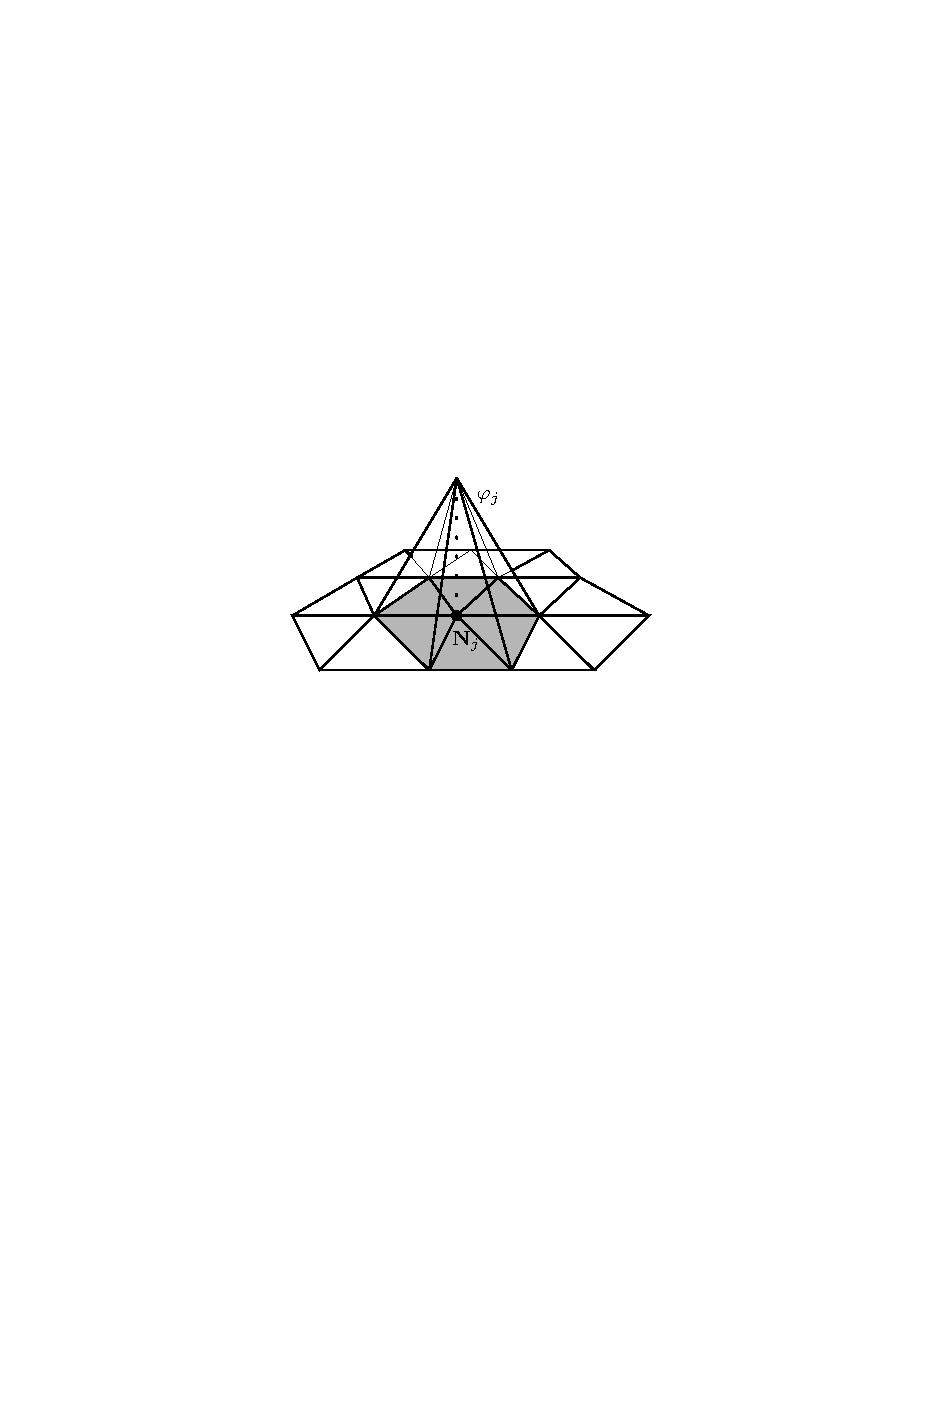
\includegraphics[width=0.5\textwidth]{tria_basis}
\caption{Piecewise affine basis functions}
\end{center}
\end{figure}
We will take the control to be of the form
\[
u(y,t) = v(t) \sin(\pi y)
\]
Then the finite element solution is of the form
\[
z(x,y,t) = \sum_{j \in N_f} z_j(t) \phi_j(x,y) + v(t) \sum_{j \in N_c} \sin(\pi y_j) \phi_j(x,y)
\]
The approximate weak formulation is given as
\[
 \dd{}{t}(z(t), \phi_i)_{L^2} = - \mu \int_\Omega \nabla z \cdot \nabla \phi_i \ud x +  \alpha \int_\Omega z \phi_i \ud x, \quad \forall i \in N_f
\]
i.e.,
\begin{eqnarray*}
&& \sum_{j \in N_f} \dd{z_j}{t} \int_\Omega \phi_j \phi_i + \dd{v}{t} \sum_{j \in N_c} \sin(\pi y_j) \int_\Omega \phi_j \phi_i \\
&=& -\mu \sum_{j \in N_f} z_j \int_\Omega \nabla \phi_j \cdot \nabla \phi_i - \mu v \sum_{j \in N_c} \sin(\pi y_j) \int_\Omega \nabla \phi_j \cdot \nabla \phi_i \\
&& + \alpha \sum_{j \in N_f} z_j \int_\Omega \phi_j \phi_i + \alpha v \sum_{j \in N_c} \sin(\pi y_j) \int_\Omega \phi_j \phi_i, \qquad \forall i \in N_f
\end{eqnarray*}
In order to simplify the presentation we will ignore the term containing $\dd{v}{t}$\footnote{This term vanishes if we use the trapezoidal rule for integration.} and then we can write the FEM formulation as
\begin{eqnarray*}
&& \sum_{j \in N_f} \dd{z_j}{t} \int_\Omega \phi_j \phi_i \\
&=&  \sum_{j \in N_f} z_j \left[ -\mu\int_\Omega \nabla \phi_j \cdot \nabla \phi_i + \alpha \int_\Omega \phi_j \phi_i \right] \\
&& v \sum_{j \in N_c} \left[ - \mu  \sin(\pi y_j) \int_\Omega \nabla \phi_j \cdot \nabla \phi_i + \alpha\sin(\pi y_j) \int_\Omega \phi_j \phi_i \right] \qquad \forall i \in N_f
\end{eqnarray*}
This can be written as a system of ordinary differential equations
\[
 \M \dd{\z}{t} = \A \z + \B v
\]
where $\z$ denotes all the unknown degrees of freedom in the set $N_f$.
%-----------------------------------------------------------------
\subsection{Finite element assembly}
The finite element basis functions have compact support. Hence we can compute the integrals 
\[
\int_\Omega \phi_i \phi_j \qquad \mbox{and} \qquad \int_\Omega \nabla \phi_i \cdot \nabla \phi_j
\]
by adding the contributions from a small number of triangles. For example, the elements of the mass matrix can be computed as
\[
\int_\Omega \phi_i \phi_j = \sum_{K \ : \ i, j \in K} \int_K \phi_i \phi_j
\]
and similarly the stiffness matrix is computed as
\[
\int_\Omega \nabla \phi_i \cdot \nabla \phi_j = \sum_{K \ : \ i, j \in K} \int_K \nabla \phi_i \cdot \nabla \phi_j
\]
The integrals on each triangle $K$ will be evaluated exactly. For a triangle $K$ with vertices labelled 1, 2, 3 as in figure~(\ref{fig:tria}), the local mass and stiffness matrices are given by
\[
M^K = \frac{1}{24} \mbox{det}\begin{bmatrix}
x_2 - x_1 & x_3 - x_1 \\
y_2 - y_1 & y_3 - y_1
\end{bmatrix} \begin{bmatrix}
2 & 1 & 1 \\
1 & 2 & 1 \\
1 & 1 & 2
\end{bmatrix}
\]
\begin{figure}
\begin{center}
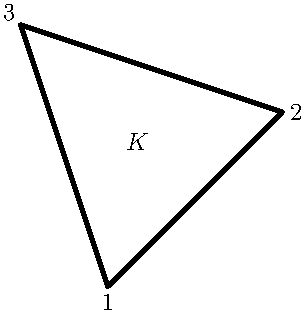
\includegraphics[width=0.3\textwidth]{tria}
\caption{Triangle}
\label{fig:tria}
\end{center}
\end{figure}
\[
A^K = \half \mbox{det}\begin{bmatrix}
1 & 1 & 1 \\
x_1 & x_2 & x_3 \\
y_1 & y_2 & y_3
\end{bmatrix} G G^\top \qquad\textrm{where}\qquad G = \begin{bmatrix}
1 &  1 & 1\\
x_1 & x_2 & x_3 \\
y_1 & y_2 & y_3
\end{bmatrix}^{-1} \begin{bmatrix}
0 & 0 \\
1 & 0 \\
0 & 1
\end{bmatrix}
\]
The numerical process can be summarized by the following algorithm:

\vspace{2mm}
\noindent
Set $\M=0$, $\A=0$.\\
For each triangle $K$ in the mesh
\begin{itemize}
\item Compute $M^K$ and $A^K$
\item Add the contributions from $M^K$ into $\M$ and from $A^K$ into $\A$
\end{itemize}
More details on the assembly process can be found in this paper

\vspace{2mm}\noindent
Jochen Alberty, Carsten Carstensen and Stefan A. Funken: ``Remarks around 50 lines of Matlab: short finite element implementation", Numerical Algorithms 20 (1999) 117�-137\\
\url{http://math.tifrbng.res.in/~praveen/notes/control2013/acf.pdf}
%-----------------------------------------------------------------
\subsection{Computing the observation}
We will assume that the intervals $[a_i, b_i]$ on which the observation is computed is exactly covered by the edges of the finite element mesh. Let $E_i$ denote the edges on $[a_i,b_i]$
\begin{eqnarray*}
y_i &=& \frac{1}{b_i-a_i} \int_{a_i}^{b_i} z(0,y,t) \ud y \\
&=& \frac{1}{b_i-a_i} \sum_{e \in E_i} \int_e z(0,y,t) \ud y \\
&=& \frac{1}{b_i-a_i} \sum_{e \in E_i} \half (z_{e_1} + z_{e_2}) |e|
\end{eqnarray*}
The set of observations can be written as
\[
\y = \bH \z
\]
The observation zones are defined by the following parameters
\begin{center}
\begin{tabular}{|c|c|c|c|}
\hline
Value/$i$ & 1 & 2 & 3 \\
\hline
$a_i$ & 0.20 & 0.50 & 0.80 \\
\hline
$b_i$ & 0.25 & 0.55 & 0.85 \\
\hline
\end{tabular}
\end{center}
%-----------------------------------------------------------------
\subsection{Grid information}
The grid information consists of following files
\begin{itemize}
\item {\tt coordinates.dat}: contains $x,y$ coordinates of all the vertices

\item {\tt elements3.dat}: contains verices forming each triangle

\item {\tt dirichlet.dat}: contains boundary edges on the dirichlet boundary

\item {\tt neumann.dat}: contains boundary edges on the neumann boundary

\end{itemize}
An example of this type of data is given in figures~(\ref{fig:fem501}),~(\ref{fig:fem502}). In each file, the first column is the serial number.
\begin{figure}
\begin{center}
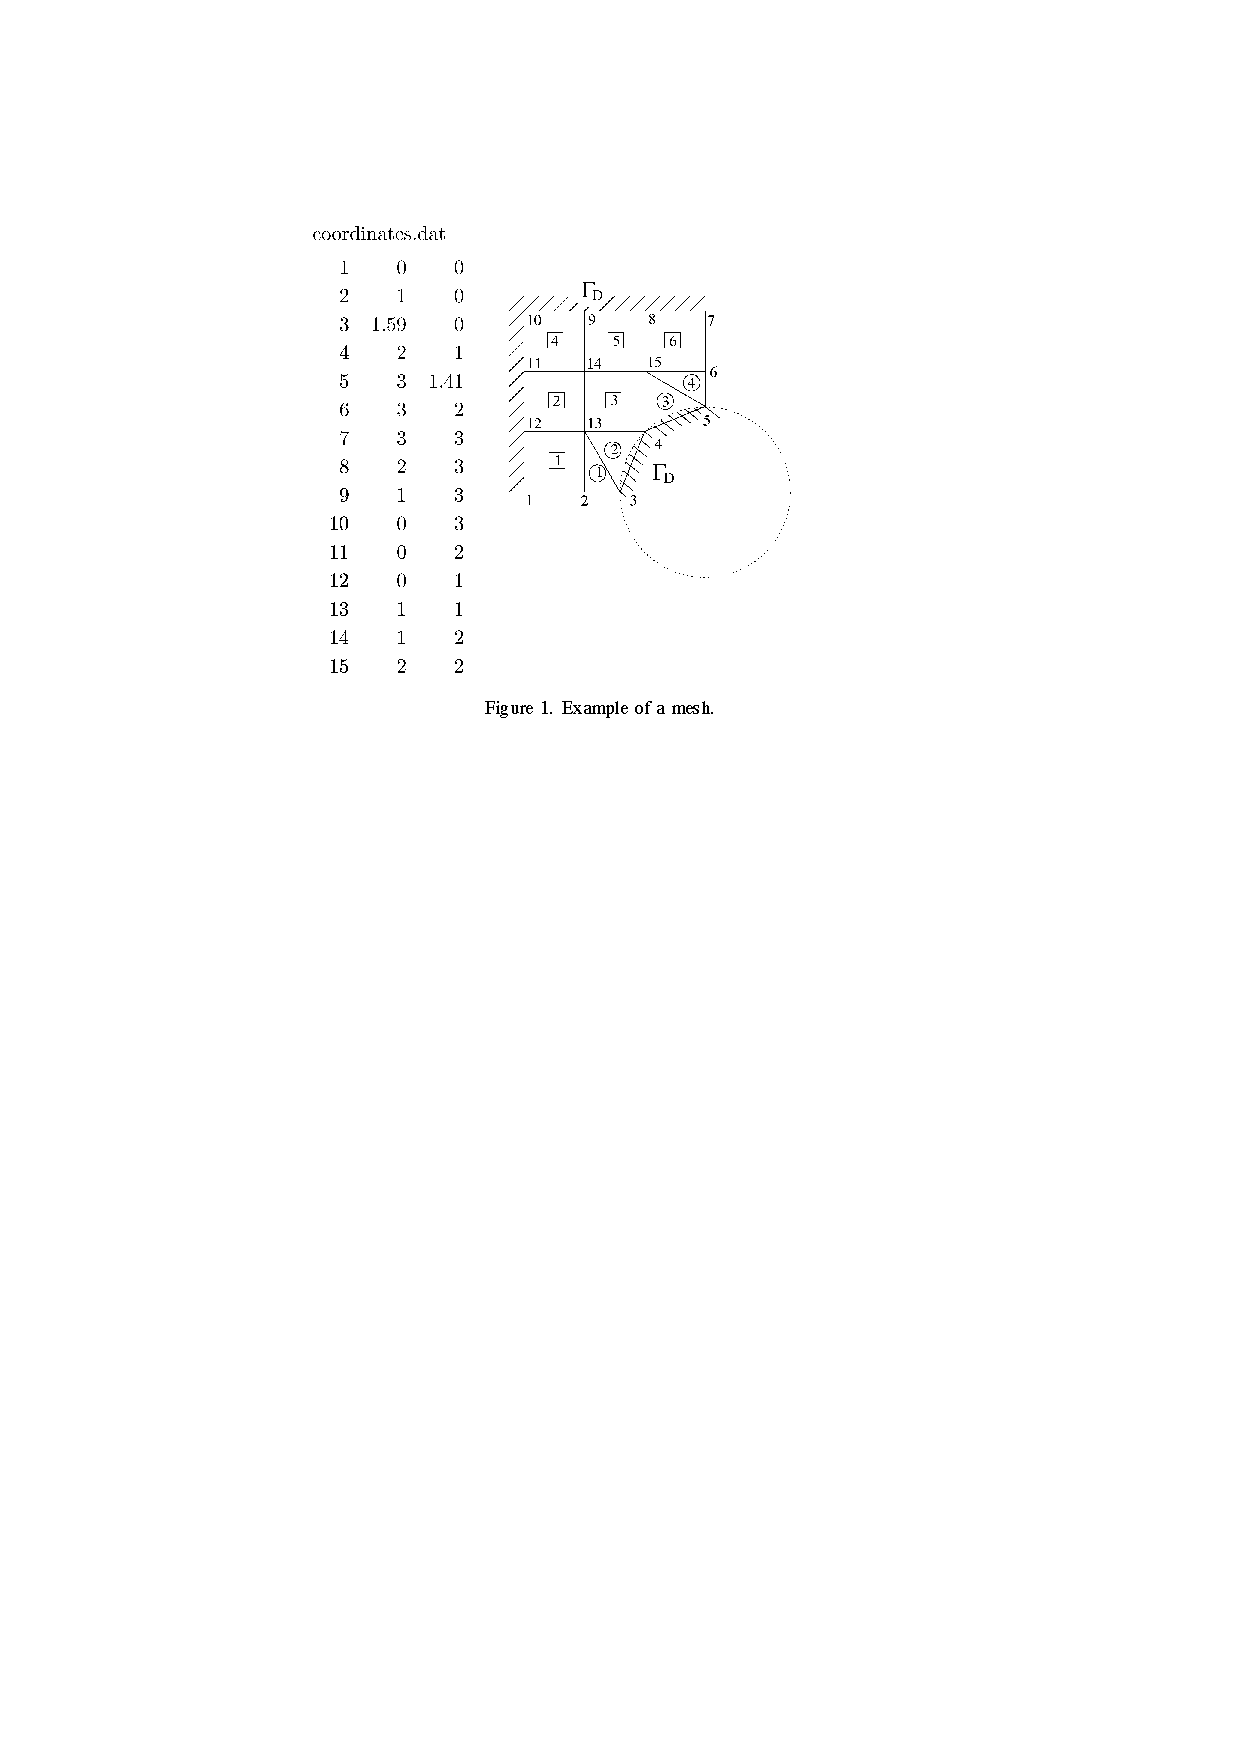
\includegraphics[width=0.7\textwidth]{fem50_1}
\caption{Example of a mesh}
\label{fig:fem501}
\end{center}
\end{figure}

\begin{figure}
\begin{center}
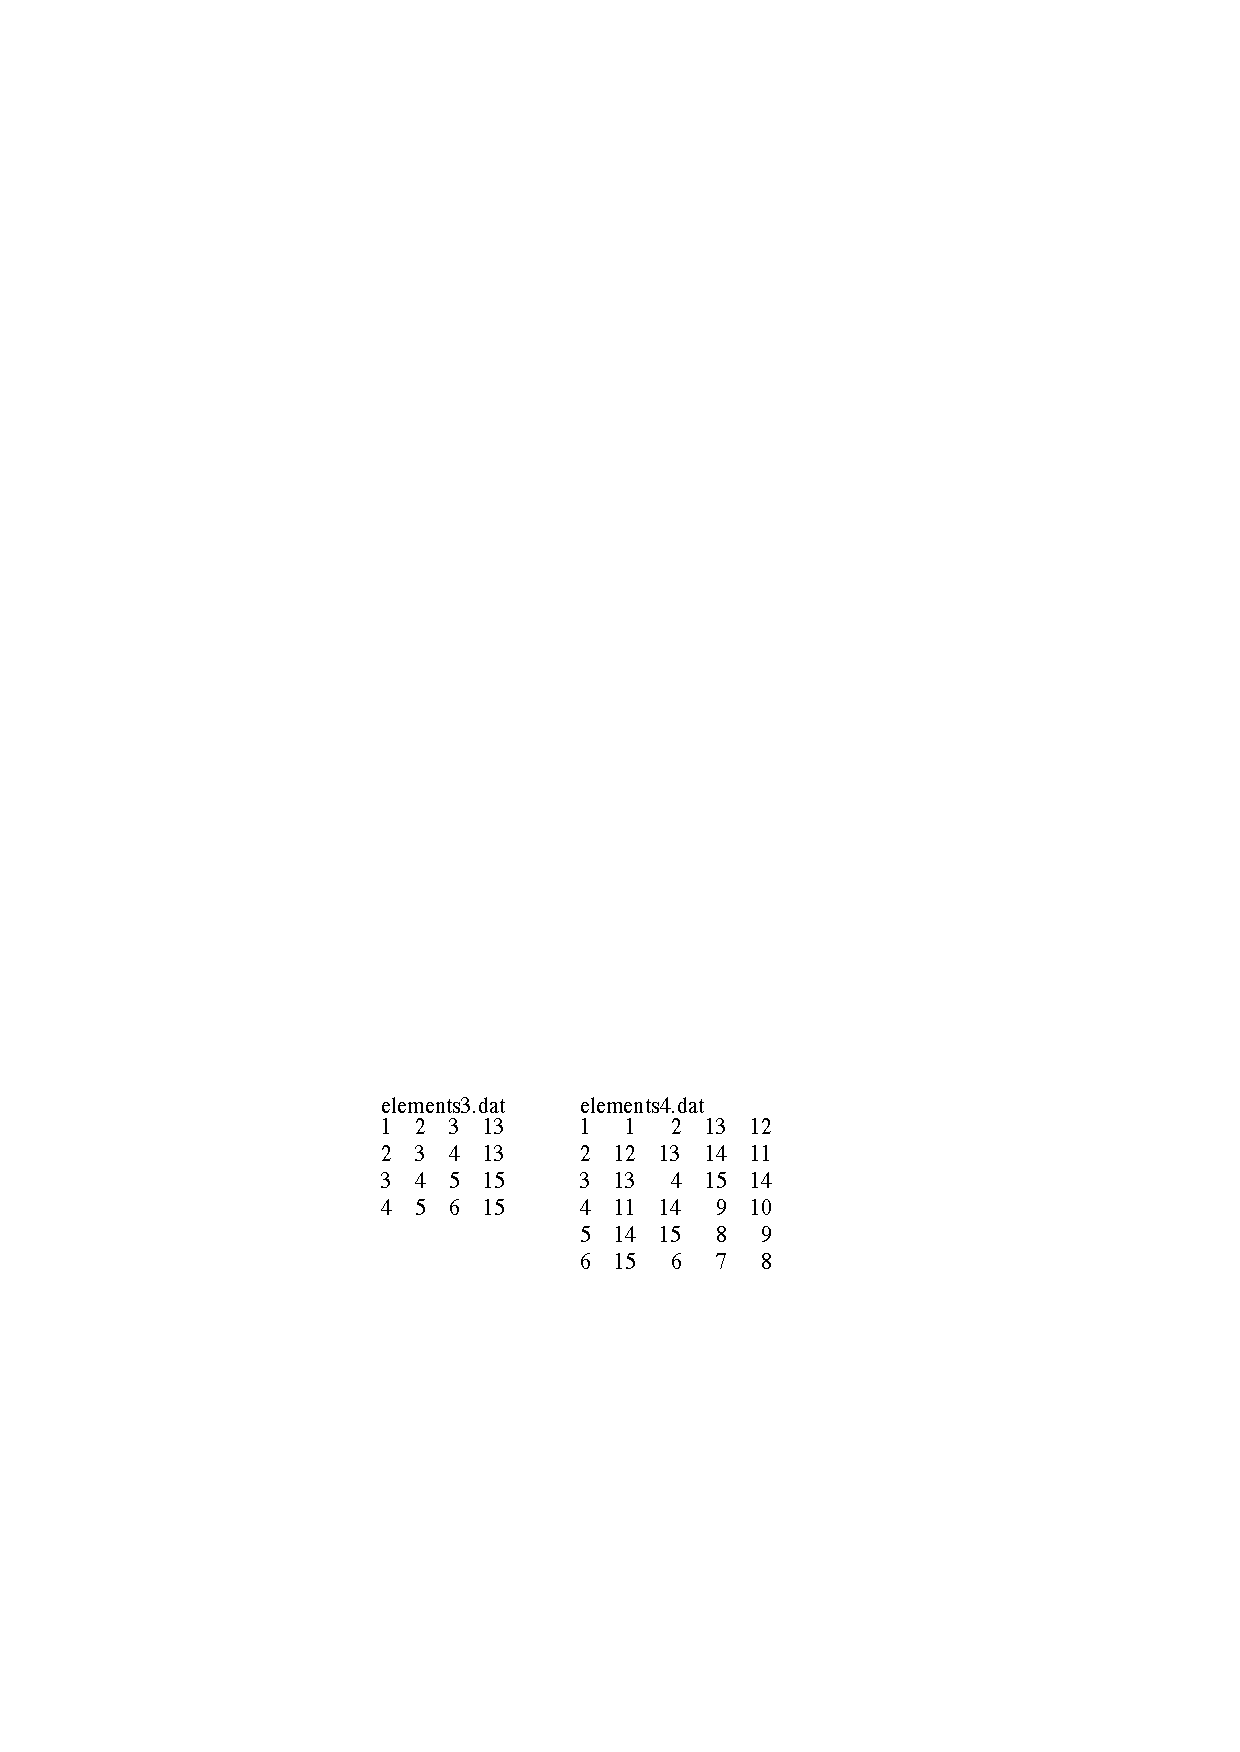
\includegraphics[width=0.5\textwidth]{fem50_2}
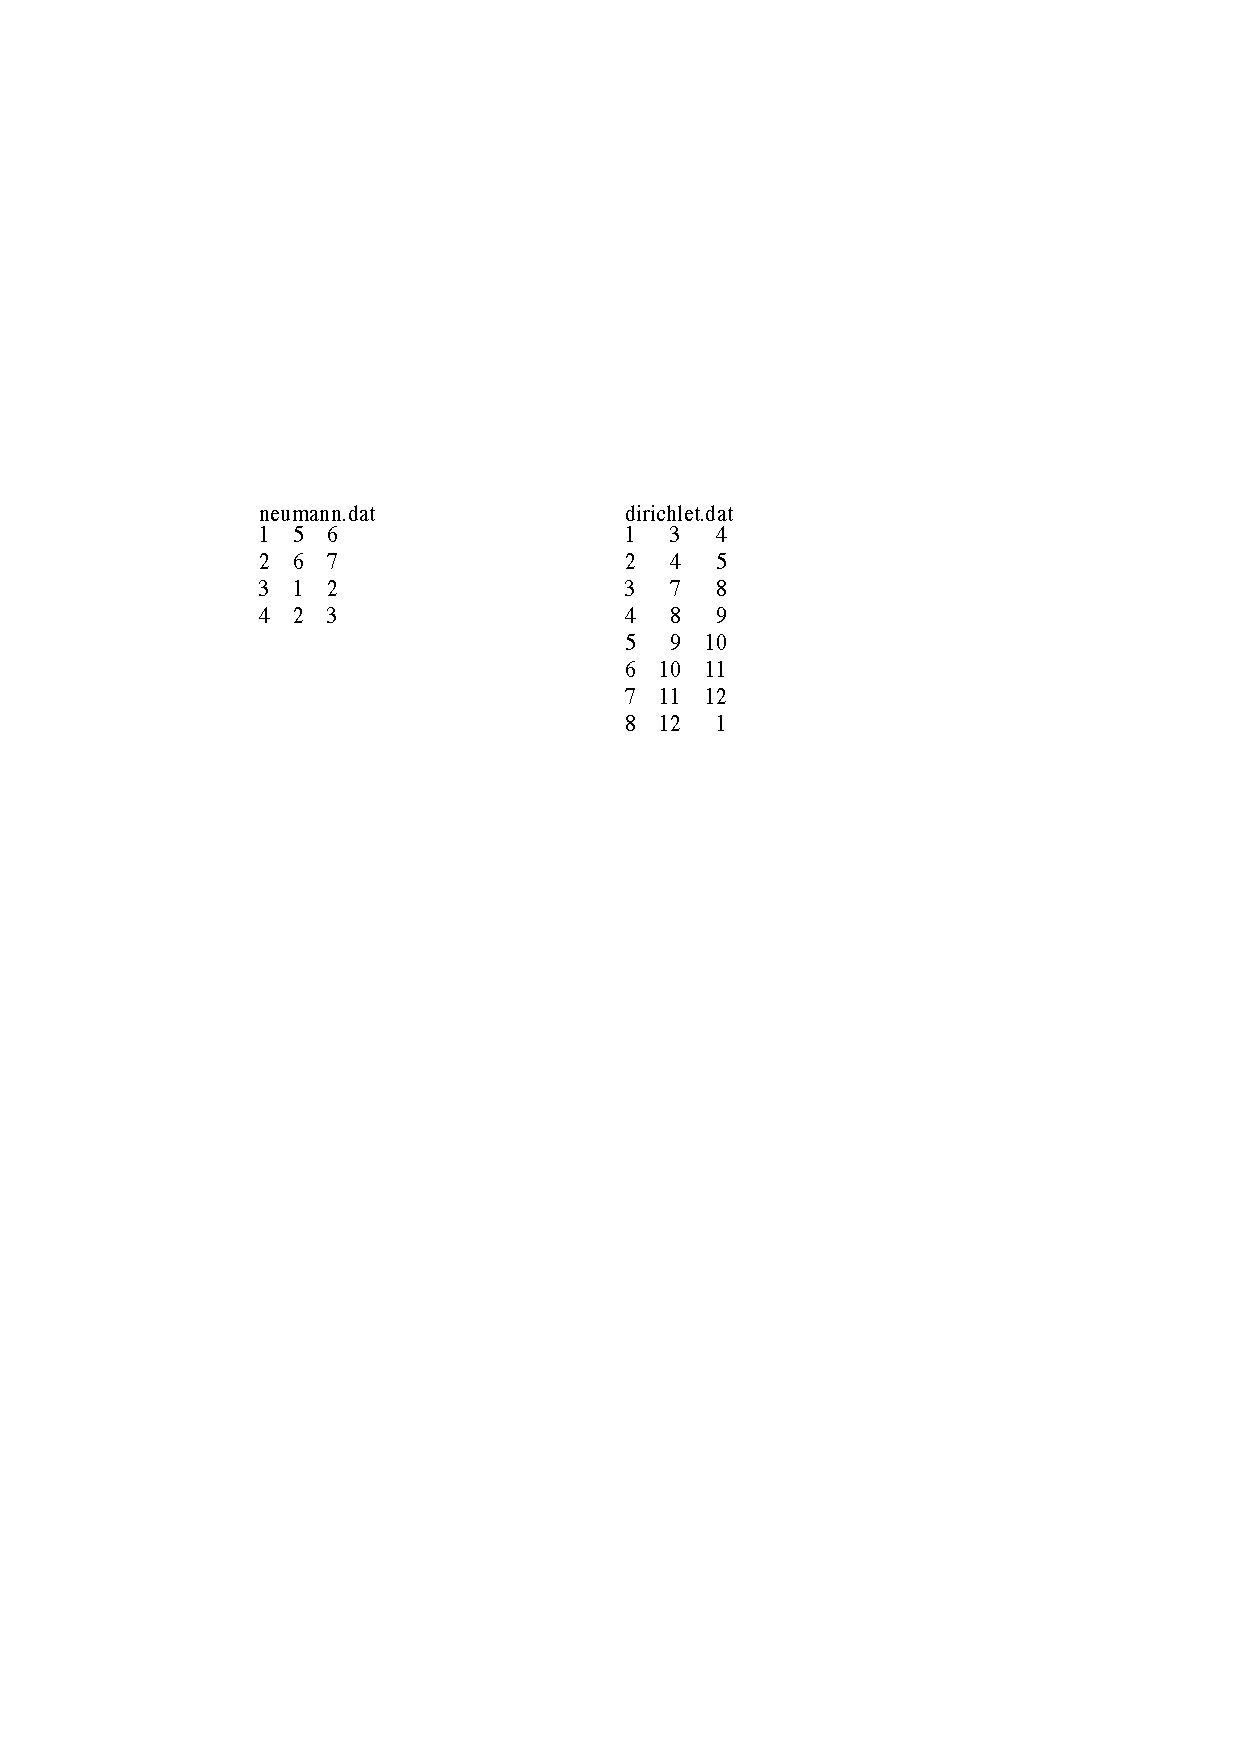
\includegraphics[width=0.6\textwidth]{fem50_4}
\caption{Structure of mesh files}
\label{fig:fem502}
\end{center}
\end{figure}

\begin{center}
{\bf Note: In our current programs we use a mesh consisting of only triangles. \\
Also, the serial numbers are not stored in the files. }
\end{center}

The domain $\Omega$ is the unit square. The program {\tt square.m} generates the mesh and creates the above four files. You have to specify the number of vertices on the side of the square. E.g., to have 11 points on each side, you do the following in matlab
\begin{lstlisting}
>> square(11)
\end{lstlisting}
When you run the above program, you can see a picture of the mesh. Examine the four files created by this program. For our actual computations, we will use 101 points on each side of the square. In this case, there are 5 edges which exactly cover each of the three observation zones.
%-----------------------------------------------------------------
\section{Estimation and feedback control}
%-----------------------------------------------------------------
\section{List of matlab programs}
%-----------------------------------------------------------------
\section{Excercises}
Let us take
\[
\mu = \frac{1}{50}, \qquad \omega = 0.1
\]
Then the heat equation has one unstable eigenvalue given by
\[
\lambda = -\frac{\pi^2}{40} + \omega =
\]
%-----------------------------------------------------------------

\end{document}  